\usetikzlibrary{calc}
\usetikzlibrary{positioning}
\usetikzlibrary{matrix}

\pgfdeclarelayer{background}
\pgfsetlayers{background,main}

\newtheorem{mydef}{Definition}
\newtheorem{algo}{Variante}

\chapterimage{chapter_head_1.png}
\chapter{Genetische Algorithmen}

\section{Intro \& Motivation}
Was bedeutet eigentlich Intelligenz?

Das ist eine Frage, auf die keiner eine absolut klare Antwort geben kann. Was wir aber mit Sicherheit wissen ist, dass wir Menschen uns als intelligent bezeichnen. Um nun also das Konzept der künstlichen Intelligenz besser zu verstehen und voran zu treiben, hat man sich -- ähnlich zu den neuronalen Netzen -- einen Ansatz überlegt, der sich an der Natur orientiert:
Genetische Algorithmen!

Dieser Typ Algorithmus verhält sich ähnlich zu den simplen Prinzipien der Genetik und wird häufig dafür genutzt, um Optimierungsprobleme zu lösen. Um euch dies näher zu bringen, werde ich im Folgenden das Prinzip, die Funktionsweise und Arbeitsbereiche von genetischen Algorithmen erläutern.

\section{Begriffe}
\begin{mydef}(Individuum)\\
	Ein Individuum ist einzelnes Element des großen Ganzen. Es ist nicht teilbar und ist das "`Ding"', was betrachtet wird. In der Biologie sind dies häufig die Zellen, aber hier werden Kandidaten für mögliche Lösungen eines Problems betrachtet.
\end{mydef}
\begin{mydef}(DNA)\\
	Die DNA ist die  Codierung sämtlicher Erbinformationen eines Individuums. Sie entspricht der Zusammenfassung aller Grundeigenschaften.
\end{mydef}
\begin{mydef}(Gen)\\
	Ein Gen ist ein Abschnitt der DNA. Es entspricht meist einer einzelnen Eigenschaft des Individuums, kann aber auch manchmal mehrere Eigenschaften umfassen.
\end{mydef}
\begin{mydef}(Population)\\
	Die Population ist die Menge aller betrachteten Individuen zu einem bestimmten Zeitpunkt.
\end{mydef}
\begin{mydef}(Genotyp/Phänotyp)\\
	Der Genotyp ist die Beschreibung eines Individuums in codierter Form. Der Phänotyp dagegen beschreibt das Individuum so, wie es ist, also durch seine Eigenschaften.
\end{mydef}
\begin{mydef}(Fitness)\\
	Die Fitness eines Individuums gibt dessen Güte/Stärke an. Von ihr hängen hauptsächlich die Überlebenschancen ab.
\end{mydef}

\section{Biologischer Hintergrund}
Im Folgenden werde ich kurz die Abläufe der Evolution auf biologischer Ebene erläutern. Dafür betrachte ich de Zellebene in Kombination mit der Vererbung, wie sie beim Menschen auftritt.

Jede Zelle hat eine eigene DNA (Desoxyribonucleinsäuren) im Kern, die sämtliche Informationen speichert. Diese ist aus verschiedenen Basenpaaren zusammengesetzt, die wie Puzzelteile ineinander passen. Die Gene sind Teilabschnitte der DNA und sind eine Codierung für je eine Eigenschaft. Bespiele sind helle Haut oder blaue Augen. Die Allele sind jeweils Paare von 2 Genen, die zu ein und derselben Eigenschaft gehören. Dabei stammt je ein Gen vom Vater und eines von der Mutter.

Es gibt verschiedene Arten von Erbgängen. Ich werde im Folgenden zunächst den dominant-rezessiven Erbgang erklären:
Dabei ist ein Gen dominant und das andere rezessiv, was bedeutet, dass sich das dominante durchsetzt und letztendlich für die bestimmte Eigenschaft verantwortlich ist. Es sind aber beide Gene in der DNA enthalten. Bei der Reproduktion wird sowohl beim Vater, als auch der Mutter von jedem Allel eines der Gene ausgewählt und dann zu einem neuen Allel kombiniert. Dies kann dazu führen, dass beispielsweise zwei rezessive Gene zusammenkommen und sich dann im Kind eine Eigenschaft durchsetzt, die keines der beiden Elternteile besaß.

Nun folgt der intermediäre Erbgang:
Hierbei haben die Gene verschiedene Werte und bei der Vererbung überlagern sich diese. Hat man zum Beispiel zwei Blumen, von denen eine weiß und die andere rot ist, so kann die Kreuzung der beiden eine rosa Blume hervorbringen.

Es können zufällige Veränderungen in der DNA einer Zelle auftreten. Dies kann zum Beispiel durch äußere Einflüsse, wie radioaktive oder ultraviolette Strahlung auftreten. Die Zellen versuchen meist diese Veränderung rückgängig zu machen, gelingt dies jedoch nicht, so ist eine Mutation in der Zelle aufgetreten. Dies kann unter anderem auch zu Krankheiten wie Krebs führen. Die Mutationen werden auch bei der Vererbung weitergegeben.

Die Selektion basiert auf dem Überleben des Stärkeren. Dies kann sich in vielen verschiedenen Dingen äußern. Einige Beispiele sind Anpassungsfähigkeit bei Veränderung der Umweltbedingungen, Stärke beim Kampf um Nahrung, Schnelligkeit und Wendigkeit, strategisches Handeln. Dabei kann es auch Vor- oder Nachteile durch gewisse Mutationen geben.

Ein weiterer Faktor ist hierbei auch die Nahrungskette. Die Lebewesen, die höher in der Nahrungskette stehen, setzen sich oft gegenüber den Schwächeren durch, da sie diese einfach fressen. Dies bedeutet aber nicht unbedingt, dass sie überleben, wenn sie nicht so anpassungsfähig sind, wie andere.

Beim Menschen tritt die natürliche Selektion jedoch kaum noch auf. Dies kommt daher, dass wir Menschen versuchen alle Leute aufzufangen, indem wir ein soziales Konstrukt aufgebaut haben. Dabei ist es das Ziel, dass jeder mit den lebensnotwendigen Dingen versorgt wird und eine Chance hat sich in die Gesellschaft einzubringen.

\section{Ablauf}
Das Ziel eines genetischen Algorithmus ist die Optimierung der Fitness aller Individuen in einer Population. Dies wird durch langfristige Weiterentwicklung in einem Zyklus erreicht.
Es startet mit einer Anfangspopulation, die sich durch Vererbung immer weiter entwickelt. Man fängt damit zunächst mit einer Betrachtung des Genotyps an.

Der erste Schritt ist die Mutation einzelner Stellen in den Genen der Individuen.
Darauf folgt dann eine Kreuzung der Individuen zu jeweils neuen Nachkommen. Dafür werden die Gene zweier Individuen zunächst aufgespalten und dann neu kombiniert. Dies kann auf verschiedene Arten geschehen. Man kann z.~B. den Anfang des ersten mit dem Ende des zweiten Gens kombinieren.
Dann wird der Phänotyp betrachtet. Dieser wird mit Hilfe einer Fitness-Funktion bewertet und anhand dieser, werden die Überlebenschancen für ein Individuum festgelegt.
Zuletzt findet dann die Selektion statt. Dabei werden aus sämtlichen neu entstandenen Individuen die "`besten"' ausgewählt, um die nächste Generation zu bilden. Mit dieser kann dann wieder von vorne begonnen werden.

Dies wird solange wiederholt, bis man sein Ziel erreicht hat oder es keinen Fortschritt mehr zu beobachten gibt. Dies kann aufgrund verschiedener Probleme, die später noch genauer erläutert werden, auftreten.

\section{Codierung}
Um die Individuen gut betrachten und später reproduzieren zu können muss man eine anschauliche Darstellung für die Gene wählen. Diese Wahl hängt hauptsächlich vom gegebenen Problem ab und kann deshalb nicht allgemein angegeben werden. Dennoch werde ich einige grundlegende Prinzipien zur Codierung darstellen.

\subsection{Binärcodierung}
Die Binärcodierung ist eines der ältesten Konzepte und beruht auf der Darstellung von Zahlen im Binärsystem. Dabei haben die Gene immer eine feste Länge und die Stellen darin sind entweder 0 oder 1. Die Bedeutung der Gene lässt sich im Genotyp zunächst nicht erkennen (dies ist im Allgemeinen unabhängig von der Codierung), kann aber nach der Umwandlung in den Phänotyp erkannt werden. So kann zum Beispiel eine 1 an einer Stelle dafür stehen, dass das Individuum eine bestimmte Eigenschaft besitzt, und eine 0, dass diese nicht vorhanden ist. Ein anderes Beispiel ist, dass die Gene einfach als Binärzahlen interpretiert werden und sich somit eine Zahl als Phänotyp ergibt.

Die Binärcodierung in Kombination mit der Interpretation als Zahlen kann aber auch zu Problemen führen. Mutiert man zum Beispiel bei einer 10-stelligen Binärzahl die erste Stelle erreicht man eine Änderung von 512 im Ergebnis, bei einer Mutation in der letzten Stelle jedoch nur um 1. Daher haben die Mutationen eine stark schwankende Bedeutung im Ergebnis zu Folge. Um dies auszugleichen bräuchte man einen großen algorithmischen Aufwand.

Ein weiterer Kritikpunkt ist, dass bei Kreuzungen das Elternteil, das für den vorderen Teil zuständig ist, einen deutlich höheren Einfluss auf die nächste Generation hat, als der hintere Teil. Dies sollte aber möglichst vermieden werden.

Ein Lösungsansatz für diese beiden Probleme ist die Verwendung des Gray Codes. Dieser hat im Gegensatz zum Binärcode den Vorteil, dass benachbarte Codewörter eine Hamming-Distanz von 1 haben, sich also zwei benachbarte Zahlen im Phänotyp, im Genotyp an nur einer einzigen Stelle unterscheiden.

\subsection{Realzahl Codierung}
Bei dieser Art der Codierung werden die Gene als reelle Zahlen aufgefasst. Im Gegensatz zur Binärdarstellung ist die Länge der Gene hier -- zumindest theoretisch -- nicht fest. In der Umsetzung ist es oft aber leichter eine feste Länge zu verwenden, was dann zu einer Darstellung as Fließkommazahlen führt.

Diese Darstellung wird oft verwendet, wenn kontinuierliche statt diskrete Probleme betrachtet werden.


\section{Reproduktion}
Im Zuge der Reproduktion werden einerseits die Gene der einzelnen Individuen mutiert und andererseits zwei Individuen zu einem neuen gekreuzt. Dabei gibt es mehrere Faktoren zu beachten, die im Folgenden erläutert werden:
\subsection{Kreuzung}
Da es oft mehrere Eigenschaften gibt, die zur Güte eines Individuums beitragen, aber nicht unbedingt ein einzelnes Individuum perfekt in allen Eigenschaften ist, ergibt es Sinn mehrere gute Individuen zu kombinieren. Da aber im Allgemeinen nicht klar erkennbar ist, welcher Teil des Gens für die Fitness positiv oder negativ verantwortlich ist, gibt es auch hier keine perfekte allgemeine Lösung als Schema zur Kreuzung. Ich werde aber dennoch mehrere Verfahren vorstellen:
\setcounter{algo}{0}
\begin{algo}(1-Punkt-Crossover)\\
	Bei diesem Verfahren werden die Gene der beiden Eltern an jeweils einer Stelle geteilt. Die Gene der Nachfahren ergeben sich dann dadurch, dass der erste Teil des einen Elternteils mit dem zweiten Teil des anderen kombiniert wird und umgekehrt. Wenn zum Beispiel das erste Individuum einen sehr guten ersten Teil des Gens besitzt, aber der zweite Teil des zweiten ist überragend, so kann die Kombination der beiden ein hervorragendes Ergebnis sein und die beiden Vorgänger um vieles überragen.
\end{algo}

\begin{algo}(N-Punkt-Crossover)\\
	Dies kann man als Verallgemeinerung des 1-Punkt-Crossovers verstehen. Dabei werden die Gene in mehr als 2 Teile aufgespalten und die Nachkommen erhalten dann alternierend die Teile der Eltern.
\end{algo}

\begin{algo}(Uniform Crossover)\\
	Dieses Verfahren unterscheidet sich von den beiden anderen dadurch, dass die Eltern nicht in Teile aufgespalten werden. Hierfür wird zu jeder einzelnen Stelle eine Wahrscheinlichkeit berechnet, ob sie ausgetauscht wird. Ist diese größer als 0,5 werden die Stellen getauscht und sonst nicht. Dadurch ergeben sich die Nachkommen.
\end{algo}

\begin{algo}(Mittelung)
	Dieser Algorithmus lässt sich gut bei reellwertiger oder ganzzahliger Codierung anwenden. Um von den Eltern auf einen Nachkommen zu kommen wählt man hier -- ähnlich zum intermediären Erbgang -- jeweils das Mittel der beiden Stellen in den Genen um den Wert an der entsprechen Stelle im Gen des Nachkommens zu berechnen.
\end{algo}

\subsection{Mutation}
Die Mutationen sind wichtig um eine höhere Varianz in die Population einzubringen. Hat zum Beispiel die Startpopulation nur Individuen mit demselben Genotyp und die Länge der Gene ist fest, so kann ohne Mutationen keine Veränderung im Genotyp, also auch im Phänotyp stattfinden, weshalb man zu keiner Lösung des Problems kommt.

Eine Möglichkeit zur Mutation ist die Veränderung einzelner Stellen in den Genen.  Anhand einer vorher festgelegten Mutationsrate wird bestimmt, ob die betrachtete Stelle gleich bleibt, oder verändert werden soll. Tritt eine Veränderung auf, so wählt man ein anderes Codewort aus, welches nun dieser Stelle zugewiesen wird. Man kann auch die maximale/minimale Anzahl der Mutationen in einem Gen oder sogar der gesamten Population festlegen, um die Mutationen gezielt zu steuern.

Die Wahl des neuen Codeworts kann auf mehrere Arten realisiert werden. Eine Möglichkeit ist eine komplett zufällige Wahl des neuen Codeworts und eine andere eine Änderung um einen kleinen Wert.

Man sollte jedoch vorsichtig bei der Wahl der Mutationsrate sein, da sonst auch Probleme auftreten können. Wählt man die Mutationsrate zum Beispiel zu hoch, kann es sein, dass die Kreuzung der besten Individuen gar keinen Effekt mehr hat, weil sie vorher bereits zu sehr verändert wurden und sich somit deutlich verschlechtert haben.

Eine andere Variante zur Mutation der Gene ist die Mutation durch Permutation. Dabei gibt es mehrere Varianten und hier werden 3 davon kurz vorgestellt:
\setcounter{algo}{0}
\begin{algo}(Swap Mutation)\\
	Hierbei werden zunächst zufällig 2 Positionen im Genotyp bestimmt und dann die Werte an den Stellen getauscht.
\end{algo}
\begin{algo}(Insert Mutation)\\
	Man bestimmt wieder 2 zufällige Positionen. Dann wird der Wert an der 2. Position direkt hinter den an der 1. verschoben und die restlichen werden jeweils um eine Position nach hinten verschoben, bis man an der 2. Position angelangt ist. Eine Voraussetzung dafür ist, dass die erste Position vor der zweiten liegt.
\end{algo}
\begin{algo}(Scramble Mutation)\\
	Der Algorithmus wählt hier wieder zwei Stellen im Gen aus und vertauscht dann zufällig alle Positionen zwischen diesen beiden. Die anderen Stellen im Gen bleiben dabei unverändert.
\end{algo}

\section{Fitness-Funktion}
Die Fitness-Funktion ist einer der wesentlichsten Bestandteile eines genetischen Algorithmus. Sie bewertet die Brauchbarkeit eines Individuums bezüglich des zu lösenden Problems und ist notwendig um später die Überlebens-/Fortpflanzungschancen festzulegen. Eine der gängigsten Varianten ist, die proportionale Fitness $\frac{B_x}{B_{gesamt}}$, die die Brauchbarkeit $B_x$ eines Individuums x in direkte Proportion zur Brauchbarkeit aller Individuen setzt. Da die genaue Form dieser Funktion stark vom zu lösenden Problem abhängt, kann man jedoch keine allgemeine Form angeben. Daher ist die Definition einer geeigneten Fitness-Funktion auch eines der größten Probleme beim Entwurf eines genetischen Algorithmus. Man kann jedoch im Allgemeinen sagen, dass es sinnvoll ist, keine Werte kleiner als 0 zuzulassen, da es sonst, wie wir später sehen werden, leicht zu Problemen kommen kann.

Man kann die Fitnessfunktion auch anpassen, um die Bedingungen zur Laufzeit des Algorithmus anzupassen:

So kann man die Fitnessfunktion $f$ zum Beispiel zeitabhängig machen, indem man $f^*=f^{k(t)}$ als neue Fitnessfunktion wählt. Der zeitabhängige Exponent k(t) steuert dann den Selektionsdruck, bewirkt also eine Anpassung der Verteilung der Überlebenswahrscheinlichkeit.

Eine weitere Variante dafür ist die sogenannte Boltzmann-Selektion. Dabei wählt man als neue Fitnessfunktion $f^*=exp(\frac{f}{kT})$. Dabei ist $T$ ein zeitabhängiger Temperaturparameter. Er fängt bei einem relativ hohen Wert an und fällt dann immer weiter ab. Dies hat zur Folge, dass mit steigender Zeit immer größere Unterschiede in der Fitnessfunktion auftreten, wodurch der Selektionsdruck immer weiter gesteigert wird. $k$ ist dabei eine Normierungskonstante.

\section{Selektion}
Wir haben nun bereits die Individuen nach ihrer Fitness bewertet, aber nun stellt sich die Frage:
Wie wirkt sich das eigentlich aus?

Es gibt verschiedene Ansätze von der Fitness zur Überlebenswahrscheinlichkeit zu kommen und ich möchte euch drei davon vorstellen:

Im Folgenden bezeichne ich mit $f(x)$ die Fitness eines Individuums $x$ und mit $P(x)$ dessen Überlebenswahrscheinlichkeit. Dabei ist die aktuelle Population die Menge $\{x_1,x_2,\dots,x_n\}$. (Achtung! Es ist auch möglich, dass nicht nur die Kinder, sondern auch die Eltern in die nächste Generation übernommen werden. Dies nennt sich "`steady state"'.)
\setcounter{algo}{0}
\begin{algo}(Fitnessproprotionale Selektion)\\
	Eine Möglichkeit ist ein simpler Stochastischer Ansatz:
	
	$$P(x_j)=\frac{f(x_j)}{\sum_{i=1}^{n}f(x_i)}$$
	
	Dabei wird die Fitness eines einzelnen Individuums ins Verhältnis zu der Summe der Fitness aller Individuen der aktuellen Population gesetzt. Dabei ergibt sich mit geeigneter Fitnessfunktion ein Wert zwischen 0 und 1, also eine gültige Wahrscheinlichkeit und somit eine Überlebenswahrscheinlichkeit.
	
	Hierbei können jedoch mehrere Probleme auftreten:
	
	\begin{enumerate}
		\item Wenn die Fitnessfunktion negative Werte zulässt, dann könnte $P(x_j)$ undefiniert sein, weil $\sum_{i=1}^{n}f(x_i)=0$ nicht ausgeschlossen ist.
		\item Für $P(x_j)$ sind negative Werte nicht ausgeschlossen, was dann keine gültige Wahrscheinlichkeit mehr ergibt.
		\item Bei einer sehr großen Population fallen einzelne Individuen mit relativ gesehen sehr großer Fitness gegebenenfalls gar nicht auf und deren Überlebenswahrscheinlichkeit ist trotzdem sehr gering.
	\end{enumerate}
\end{algo}
Um diese Probleme zu lösen kann man nun einen etwas anderen Ansatz wählen:
\begin{algo}(Ranked-Fitness-Selection)\\
	Das Individuum mit der größten Fitness sollte die besten Überlebenschancen haben, damit ein optimaler Wert erreicht werden kann. Dafür ordnet man die Individuen zunächst in absteigender Reihenfolge nach ihrer Fitness. Dann legt man einen Startwert $P_s$ als maximale Überlebenswahrscheinlichkeit fest. Die Überlebenswahrscheinlichkeit für $x_i$ berechnet sich dann als:
	
	\begin{center}
	$P(x_i)=\begin{cases}
	P_s & \mathrm{falls~} i=1\\
	(1-P_s)P(x_{i-1}) & \mathrm{sonst}
	\end{cases}$
	\end{center}
	
	Damit erhält man in jedem Fall eine gültige Wahrscheinlichkeit und die besten Individuen haben eine deutlich höhere Überlebenswahrscheinlichkeit als der Rest.
	
	Ein Problem bleibt aber bestehen:
	Lokale Maxima in der Fitnessfunktion können schnell dazu führen, dass kein Fortschritt mehr auftritt und der Algorithmus somit nicht mehr funktioniert.
\end{algo}
Um dieses Problem zu umgehen, muss eine hohe Varianz in der neuen Population gesichert werden. Dafür kann man folgenden Ansatz verwenden:
\begin{algo}(Uniform-Fitness-Selection)\\
	Man bewertet im Folgenden nicht mehr ausschließlich nach der höchsten Fitness eines Individuums, sondern zieht dabei auch die Vielfalt der nächsten Generation in Betracht. Das optimale Ergebnis wäre also eine Population mit sehr hoher Varianz und maximaler Fitness aller Individuen. Dafür bewertet man die Individuen nach folgendem Schema:
	\begin{figure}[h]
		\includegraphics[width=0.7\linewidth]{chapters/genetic/grafik.jpg}
	\end{figure}
	
	Der Startpunkt der Linien ist hierbei oben Rechts in der Ecke, also bei einem Maximum an Varianz und Fitness, also dem besten Individuum. Dabei symbolisieren die Linien einen immer weiteren Abstand zum Optimum und damit eine schlechtere Überlebenschance. Man sieht hier auch eine gewisse Abwägung zwischen Varianz und Fitness, da zum Beispiel bei der 5. Linie ein Individuum mit einer Fitness von nahezu 0 gleich bewertet wird wie eines mit maximaler Fitness, aber einer Varianz von nahezu 0.
	
	Ein Problem, das hierbei bestehen bleibt, ist, dass durch die hohe Varianz der Algorithmus nicht wirklich konvergiert. Dies kann man lösen indem man zunächst Uniform-Fitness-Selection betreibt und danach zur Ranked-Fitness-Selection wechselt.
\end{algo}
Eine weitere Methode, um anfangs eine hohe Varianz zu haben, aber später den Algorithmus zum Konvergieren zu bringen, ist die nächste Selektionsart:
\begin{algo}(Tournament-Selection)\\
	Das Prinzip ist einfach: Man wählt eine bestimmte Anzahl an Individuen aus und lässt sie gegeneinander "antreten", was einfach bedeutet, das Individuum mit der höchsten Fitness wird in die nächste Generation übernommen. Ob es danach weiterhin an "Turnieren" teilnehmen kann oder nicht, bleibt dem Programmierer überlassen.

	Der Vorteil, den man hierbei gewinnt, besteht darin, dass man die "Turniergröße", also die Anzahl der Individuen, die gegeneinander antreten, während der Algorithmus läuft, verändern kann. Wenn man also am Anfang eine hohe Varianz beibehalten möchte, wählt man eine kleine "Turniergröße", da so die Wahrscheinlichkeit, dass auch Individuen mit geringer Fitness in die nächste Generation übernommen werden, entsprechend hoch ist. Soll der Algorithmus später dann konvergieren, kann die "Turniergröße" größer gewählt werden, damit mehr Inidividuen mit einer wirklich hohen Fitness überleben.
\end{algo}
Wenn man sich nun für eine dieser Methoden (oder gegebenenfalls einer anderen) entschieden hat, bleibt noch zu klären, wie man die erhaltenen Wahrscheinlichkeiten nutzt, um die neue Generation zu entscheiden (Tournament-Selection ausgenommen, da hier keine Wahrscheinlichkeiten berechnet werden, sondern die neue Generation sofort bestimmt wird). Häufig verwendet wird dazu folgende Methode:
\begin{algo}(Roulette-Wheel-Selection)\\
	Man simuliert ein Glücksrad, welches in n Abschnitte unterteilt ist, wobei jeder Abschnitt einem Individuum zugeordnet ist und die Größe des Abschnittes des Wahrscheinlichkeit entspricht, dass das zugehörige Individuum in die nächste Generation übernommen wird. Dieses Glücksrad wird dann n mal gedreht und somit die nächste Population bestimmt.
	\begin{figure}[h]
		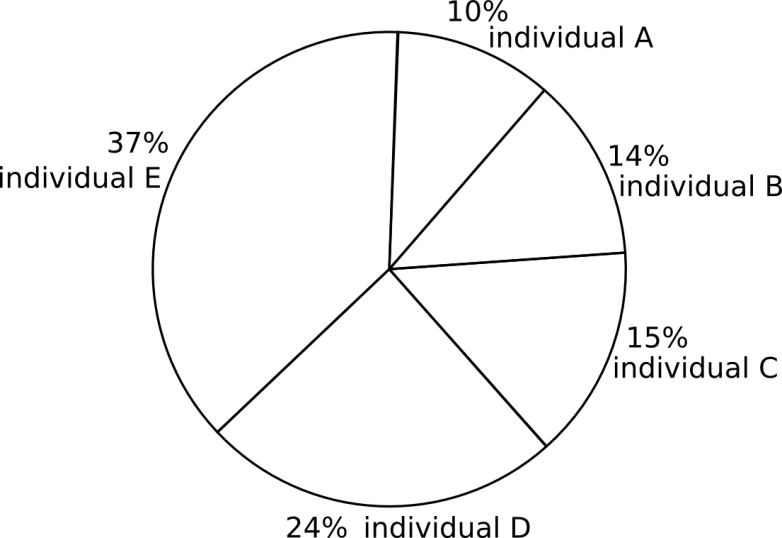
\includegraphics[width=0.7\linewidth]{chapters/genetic/rouletteWheel.png}
	\end{figure}
	
\end{algo}
\section{Anwendungsbereiche}
Ein theoretisches Anwendungsbeispiel ist das sogenannte Traveling-Salesman-Problem. Es geht dabei darum, dass ein Kaufmann von seinem Warenlager aus mehrere Stationen in einer Stadt beliefern und am Ende wieder zum Lager zurückkehren möchte. Dabei soll jede Station genau einmal besucht werden. Nummeriert man die Stationen mit 1 bis n durch, so erhält man eine Codierung für die Gene als Permutationen von 1 bis n. Die Fitnessfunktion ergibt sich dann als Kehrwert der Gesamtlänge des Weges. Bei der Reproduktion muss man jedoch vorsichtig sein, damit jedes mal gültige Permutationen entstehen. Dabei bietet es sich an eine Swap-Mutation durchzuführen. Die Kreuzung zweier Individuen erweist sich als komplizierter. Hier bietet es sich an ein Crossover durchzuführen, dann auf Gültigkeit zu testen und falls diese nicht vorhanden ist, das ganze rückgängig zu machen. Die entsprechenden Wahrscheinlichkeiten erhält man durch systematisches Probieren. Für die Selektion bietet sich dann die Ranked-Fitness-Selection an.

Genetische Algorithmen werden beispielsweise angewendet bei:
\begin{itemize}
	\item Konstruktion von komplexen Bauteilen
	\item Erstellung von Phantombildern
	\item Flugzeugbau
	\item Logistik (Ablaufplanung)
	\item Routenplanung
	\item Anordnungsprobleme
	\item Packprobleme
	\item Strategieprobleme (Spieltheorie)
	\item Parameteroptimierung
	\item Allgemein Optimierungsprobleme
\end{itemize}

Ein Beispielprogramm für die Logistik findet sich auf \href{http://www.dna-evolutions.com}{www.dna-evolutions.com}.

\section{Abgrenzung / Vergleich zu Neuronalen Netzen}
Ein Neuronales Netz ist ein Ansatz zur Lösung eines spezifischen Problems. Der Nachteil ist, dass man die Gewichte der einzelnen Knoten manuell durch Training anpassen muss. Genetische Algorithmen dagegen sind ein viel allgemeineres Prinzip, dass selbst optimale Lösungsansätze findet. So kann zum Beispiel auch ein genetischer Algorithmus verwendet werden, um ein neuronales Netz zu optimieren, oder sogar selbst zu entwerfen, indem er die Anzahl an Koten, Verbindungen und die Gewichte optimiert.\\

\section{Fazit \& Bewertung}
Genetische Algorithmen sind eine gute Möglichkeit um Optimierungsprobleme und Suchen mit großem Lösungsraum zu berechnen. Dabei werden im Gegensatz zu Expertensystemen keine weiteren Datenbanken oder ähnliches benötigt, sondern der Algorithmus verbessert sich immer weiter selbst. Der Nachteil ist, dass man in jedem  einzelnen Schritt stark vom Problem abhängige Wahlen treffen muss, die sich nicht unbedingt verallgemeinern lassen. Diese wirken sich dann stark auf den Ablauf des Programms aus und bestimmen das Ergebnis. Außerdem muss das Programm gegebenenfalls zur Laufzeit angepasst werden, entscheidet man  sich zum Beispiel das Selektionsverfahren zu ändern, damit eine Konvergenz des Algorithmus auftritt oder eine frühzeitige Konvergenz bei lokalen Maxima verhindert wird. Dennoch sind genetische Algorithmen eine sehr gute Alternative zum "`Brute Force"' Ansatz, da zum Finden einer Lösung nur ein kleiner Bruchteil des gesamten Lösungsraums betrachtet werden muss und das Programm mit einer gewissen Intelligenz nach einer Lösung sucht, anstatt blind alles auszuprobieren. Ein Problem bleibt jedoch, welches ist, dass immer nur eine Approximation und keine exakte Lösung berechnet wird. Daher muss man vorher abwiegen, ob dies ein guter Ansatz ist.

\section{Quellen und Literatur}

\href{http://www2.cs.uni-paderborn.de/cs/ag-klbue/de/courses/ws04/ea/students/ga_report.pdf}{(Skript Uni Paderporn)}\\
\href{http://www.mathematik.tu-dortmund.de/papers/MehmetiAmreinKulmsMacinLoenserBogonosWaidhas2014.pdf}{(Skript TU Dortmund)}\\
\href{http://www.spinfo.phil-fak.uni-koeln.de/fileadmin/spinfo/ki10/Genetische_algorithmen.pdf}{(Skript Uni Köln)}\\
\href{http://www.borgelt.net/slides/ga.pdf}{(Otto-von-Guericke-Universität )}\\
\href{http://www-e.uni-magdeburg.de/harbich/genetische_algorithmen/genetische_algorithmen.pdf}{(Skript Uni Magdeburg)}\\
\href{https://www.youtube.com/watch?v=kHyNqSnzP8Y}{(Vorlesung des MIT)}\\
\href{https://www.youtube.com/watch?v=6l6b78Y4V7Y}{(Vortrag von Kickstarter)}\\
\href{http://www.spektrum.de/lexikon/neurowissenschaft/zelle/14161}{(Spektrum Artikel zu Zellen)}\\
\href{http://www.spektrum.de/lexikon/biologie/genom/27365}{(Spektrum Artikel zu Genom)}\\
\href{http://semantic-web-grundlagen.de/w/images/e/e9/IntroAI-V06.pdf}{(Semantic Web)}\\
\href{http://comcute.eti.pg.gda.pl/wp-content/uploads/2012/12/image_9_5.png}{(Roulette-Wheel-Grafik)}\\
\href{http://janmonschke.com/Genetic-Algorithms/presentation/#/}{(Slides von Jan Monschke, TSP)}\\
\href{https://en.wikipedia.org/wiki/Tournament_selection}{(Tournament-Selection)}\\
Uiform-Fitness-Grafik von Denis Krzysztala\\
